\title{How Mutation Affects the Decay of Heterozygosity}
\author{Alan R. Rogers}
\date{\today}
\frame{\titlepage}

\begin{frame}
\frametitle{Two models of mutation}
The mutation rate is $u$ per gamete per generation.
\begin{center}
\begin{tabular}{lp{0.7\textwidth}}
\textcolor{blue}{Infinite alleles} & Each mutant is an allele
  never seen before.\\[1ex]
\textcolor{blue}{$K$ alleles}      & When allele $i$ mutates, the
mutant is equally likely to be any allele other than $i$. There are
$K-1$ possibilities, each with probability $1/(K-1)$. 
\end{tabular}
\end{center}
We'll focus on the model of infinite alleles.
\end{frame}

\begin{frame}
\frametitle{Model of infinite alleles}
\begin{itemize}
\item Each mutation creates a unique mutation, which has never been
  seen before.
\item Two identical gene copies remain identical in next generation
  only if neither mutates.
\item Probability of this is $(1-u)^2$, where $u$ is the mutation
  rate.
\end{itemize}
\end{frame}

\begin{frame}
\frametitle{How drift affects gene identity} 

\textbf{Without mutation}
\[
\G' = \frac{1}{2N} + \left(1 - \frac{1}{2N}\right) \G
\]

\pause
\textbf{With mutation}
\[
\G' = (1-u)^2\left[\frac{1}{2N} + \left(1 - \frac{1}{2N}\right) \G\right]
\]
\end{frame}

\begin{frame}
\frametitle{Approximations}
\begin{eqnarray*}
(1-u)^2 & \approx & 1-2u\\
\pause
\frac{1-2u}{2N} & \approx & \frac{1}{2N}
\end{eqnarray*}
\end{frame}

\begin{frame}
\frametitle{Numerical example: $(1-u)^2 \approx 1-2u$}
\begin{center}
\begin{tabular}{ccc}
$u$ & $(1-u)^2$ & $1-2u$\\ \hline\hline
 0.100000 & 0.810000 & 0.800000\\
\pause
 0.010000 & 0.980100 & 0.980000\\
\pause
 0.001000 & 0.998001 & 0.998000\\
\pause
 0.000100 & 0.999800 & 0.999800\\
\pause
 0.000010 & 0.999980 & 0.999980\\
\pause
 0.000001 & 0.999998 & 0.999998\\
\hline
\end{tabular}
\end{center}
\end{frame}

\begin{frame}
\frametitle{Numerical example: $(1-u)/2N \approx 1/2N$}
\begin{center}
\begin{tabular}{crcc}
$u$ & $2N$ & $(1-2u)/2N$ & $1/2N$\\ \hline\hline
 0.0001 &       10 & 0.0999800 & 0.10000\\
\pause
 0.0001 &      100 & 0.0099980 & 0.01000\\
\pause
 0.0001 &     1000 & 0.0009998 & 0.00100\\
\pause
 0.0001 &    10000 & 0.0001000 & 0.00010\\
\pause
 0.0001 &   100000 & 0.0000100 & 0.00001\\
\hline
\end{tabular}
\end{center}
\end{frame}


\begin{frame}
\textbf{Before approximations}
\[
\G' = (1-u)^2\left[\frac{1}{2N} + \left(1 - \frac{1}{2N}\right) \G\right]
\]

\pause
\textbf{After}
\[
\G' = \frac{1}{2N} + \left(1 - 2u - \frac{1}{2N}\right) \G\\
\]

\pause
\textbf{At equilibrium $\G' = \G$, so}\\
\pause
\fbox{\begin{minipage}{\textwidth}
\begin{eqnarray*}
\hat\G &=& \frac{1}{4Nu + 1}\\
\hat\Het &=& 1 - \hat\G = \frac{4Nu}{4Nu + 1}\\
\end{eqnarray*}
\end{minipage}}\\[5pt]
for model of infinite alleles.
The ``hats'' indicate that these are equilibrium values.
If $4Nu$ is large, $\hat\Het \approx 1$.
\end{frame}

\begin{frame}
\frametitle{Model of 2 alleles}
\[
\hat\Het = \frac{4Nu}{8Nu + 1}
\]
If $4Nu$ is large, $\hat\Het \approx 1/2$.
\end{frame}

\begin{frame}
\frametitle{History of human population size}
{\centering
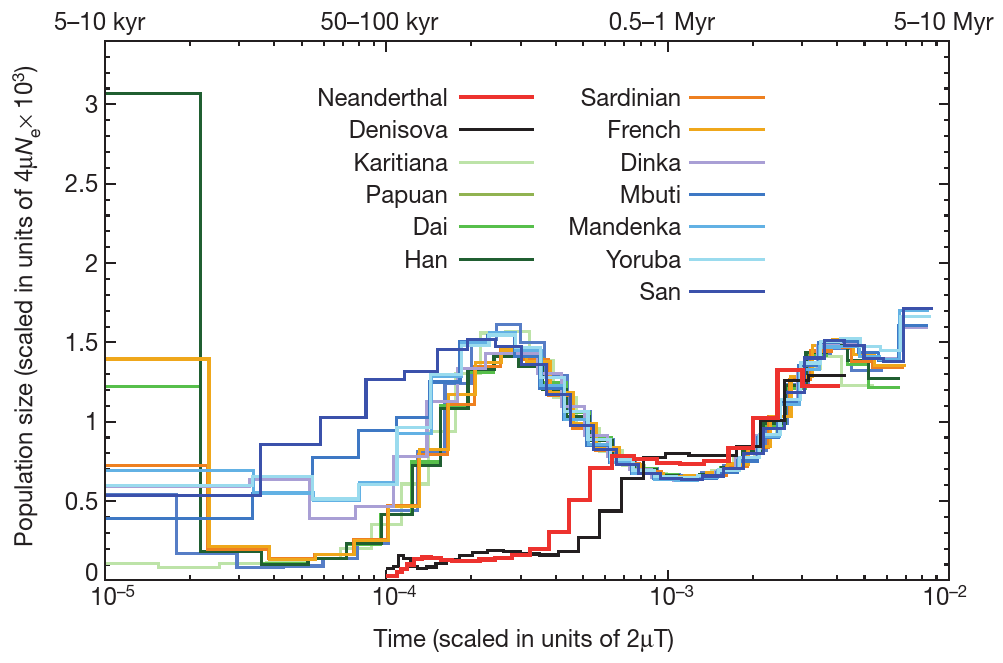
\includegraphics[width=\linewidth]{Prufer-pophist.png}\\}
\end{frame}
\begin{frame}
\frametitle{Neanderthals had low heterozygosity}
{\centering
\begin{tabular}{llr}
Species & Population & Heterozygosity\\
\hline
Neanderthal     & El Sidr{\'o}n & 0.000143\\
                & Vindija       & 0.000127\\
                & Altai         & 0.000113\\[1ex]
Modern          & African       & 0.000507\\
                & European      & 0.000387\\
                & Asian         & 0.000358
\end{tabular}\\[2ex]}

Low heterozygosity $\Rightarrow$ small population.
\end{frame}

\begin{frame}
\frametitle{The magnitude of predicted effects on heterozygosity at a
  biallelic locus}
{\centering\begin{tabular}{rr}
$N$ & $H$\\
\hline
    1,000 & 0.00004\\
   10,000 & 0.00040\\
  100,000 & 0.00400\\
1,000,000 & 0.03700\\
\hline
\multicolumn{2}{c}{$u = 10^{-8}$}\\
\end{tabular}\\}

\bigskip
Populations of different size should differ enormously in
heterozygosity. 

\pause

Is this really true?
\end{frame}

\begin{frame}
\centering%
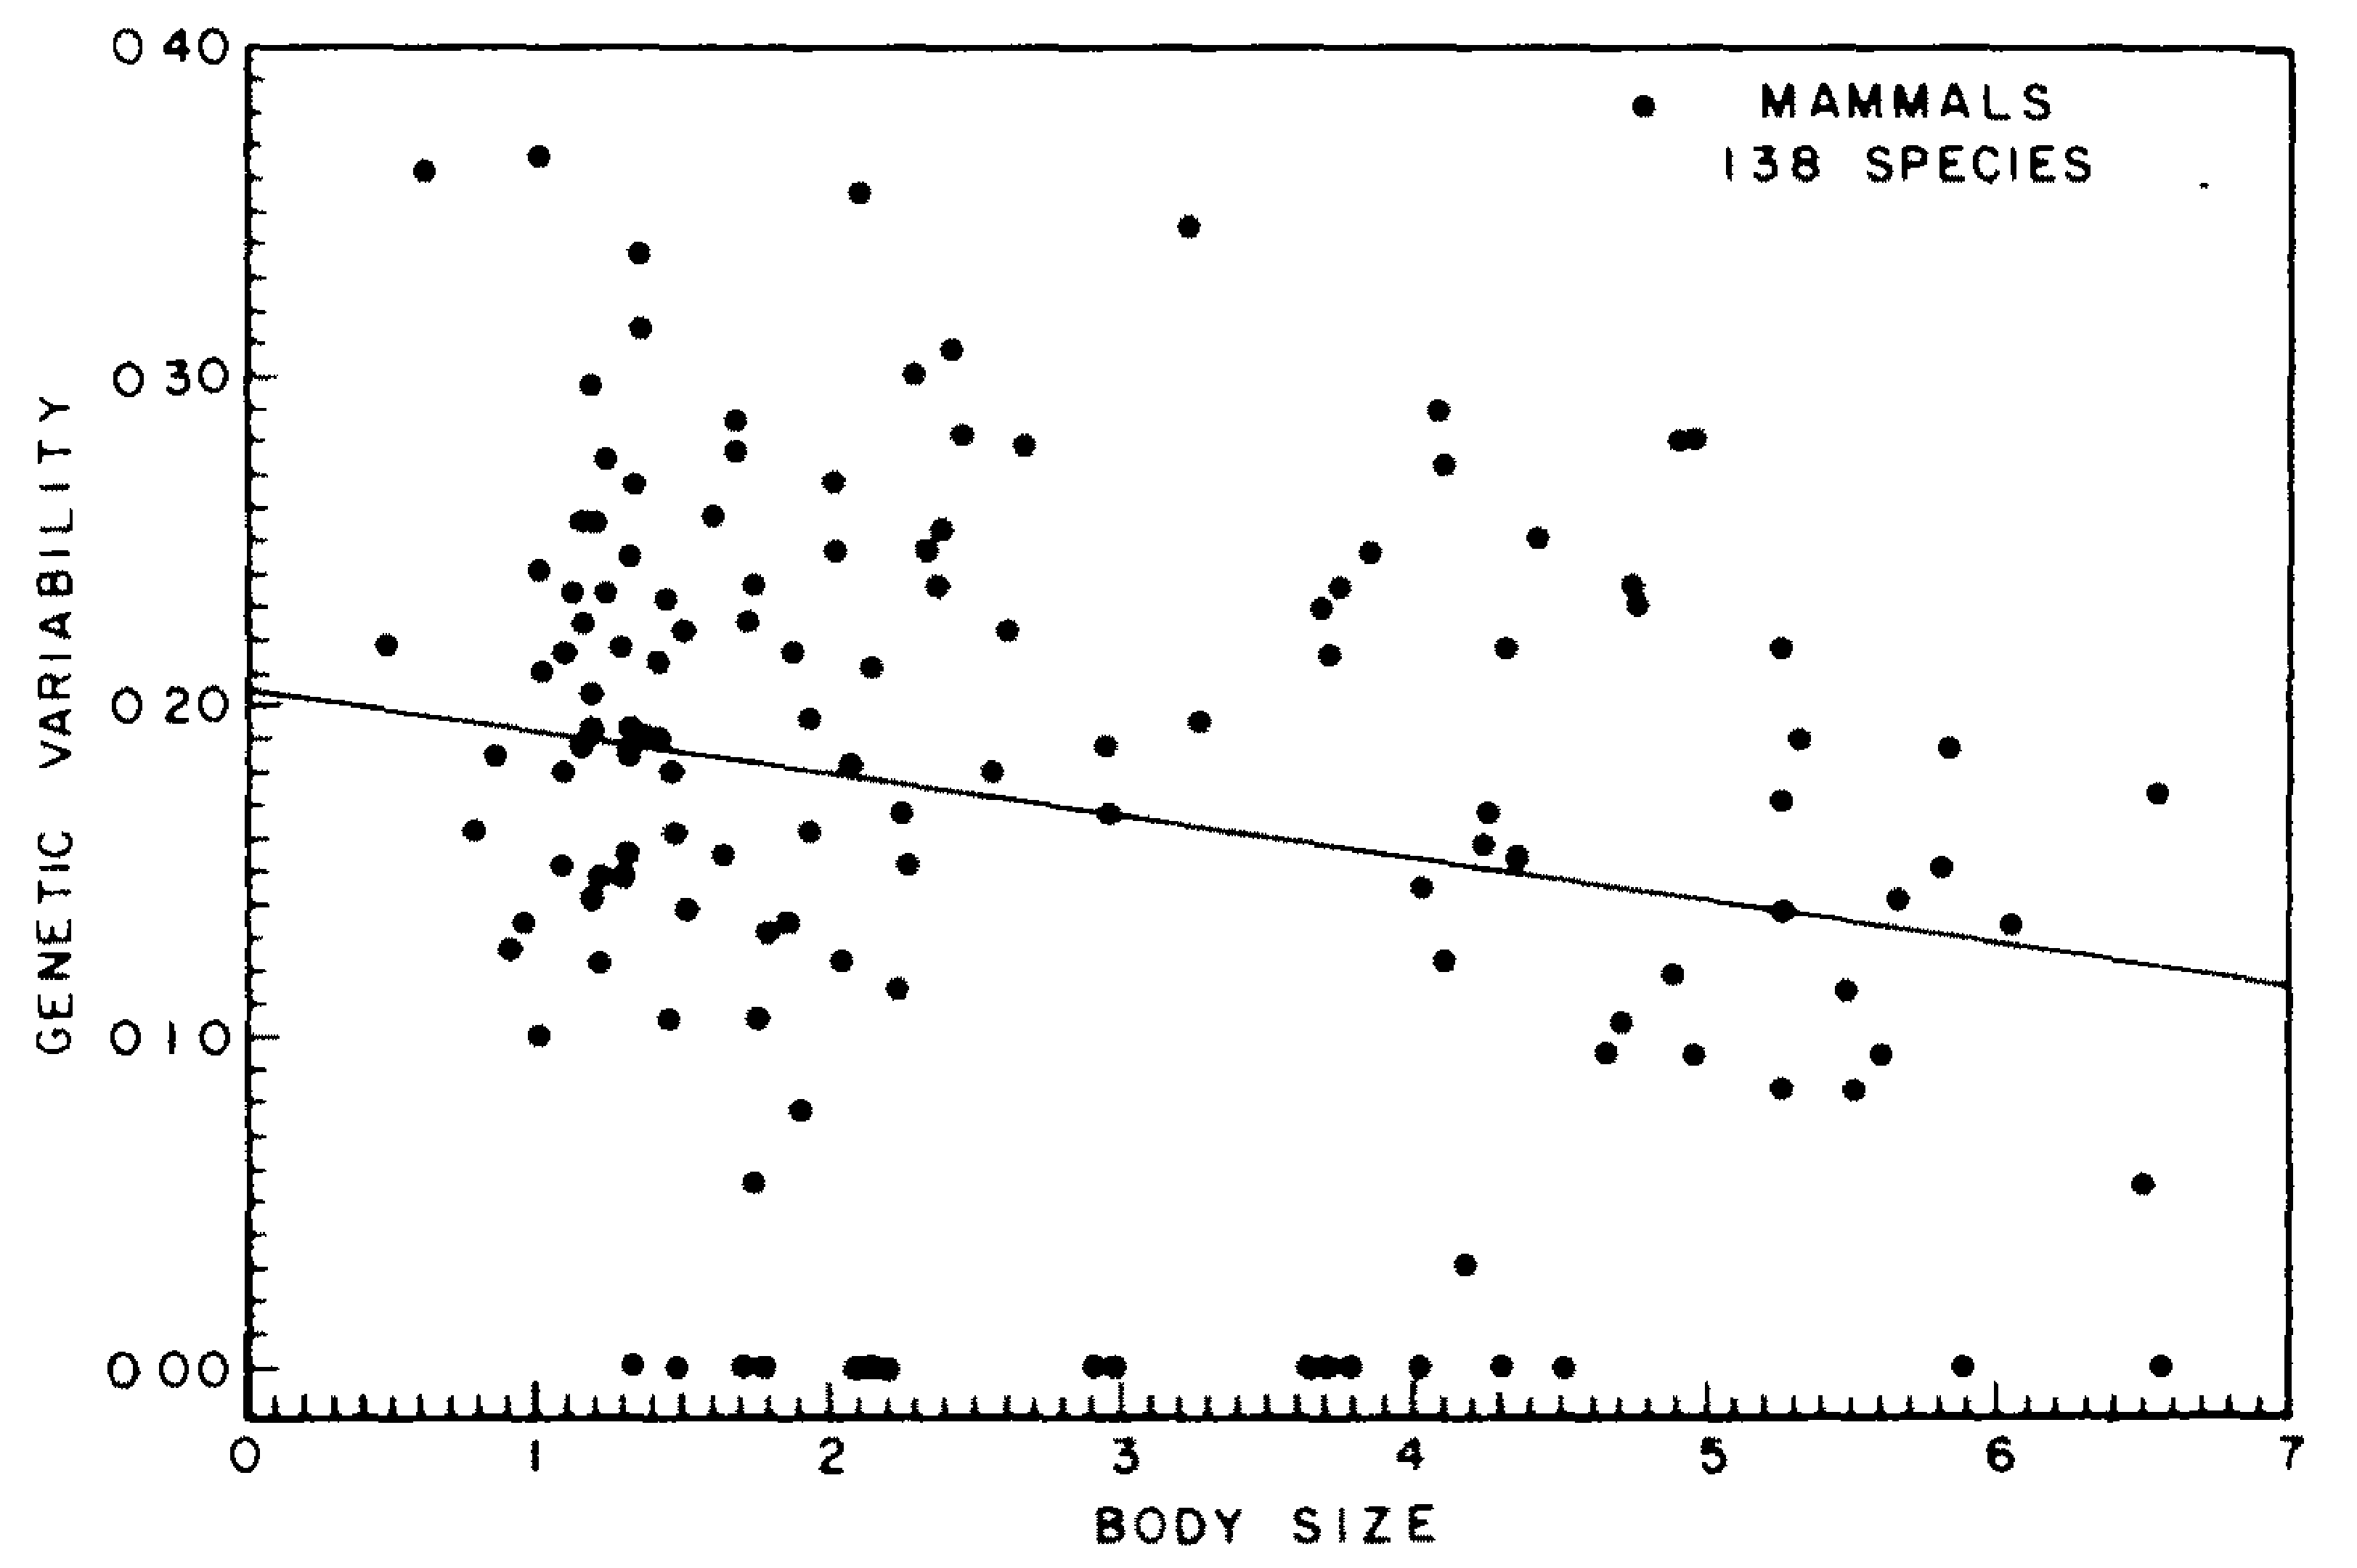
\includegraphics[width=\textwidth]{wooten-hetz.pdf}\\
Heterozygosity at enzyme polymorphisms vs $\log_{10}$ grams of body wgt
(Wooten \& Smith 1985). Range: 3~g to 4000~kg.
\end{frame}

\begin{frame}
\begin{columns}
\column{0.55\textwidth}
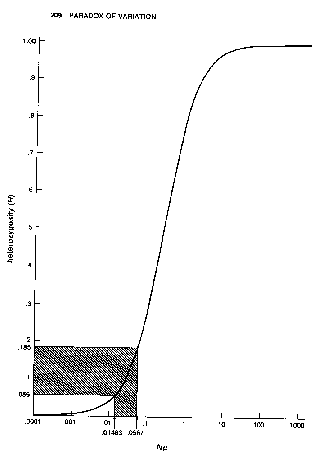
\includegraphics[width=\linewidth]{parodvar.png}
\column{0.45\textwidth}
Variation in $H$ implies implausibly-small variation in $N\mu$.\\[2ex]
\mbox{}\hfill {\small Lewontin (1970)\\} 
\end{columns}
\end{frame}

\begin{frame}
\frametitle{Puzzles}

\begin{itemize}
\item
Why is there so little heterozygosity?
\pause
\item
Small animals have large populations and should have high heterozygosity.
Why don't they?
\end{itemize}
\pause

\bigskip
Much of the rest of this course is about these questions.
\end{frame}

\begin{frame}[containsverbatim]
\frametitle{A Python program to calculate $\hat\Het$, using biallelic
model} 
\[
\hat\Het = \frac{4Nu}{8Nu + 1} = \frac{\theta}{2\theta + 1}
\]

\bigskip

\begin{verbatim}
# Expected heterozygosity as a function
# of theta = 4*N*u
def h(theta):
    return(theta/(2*theta + 1.0))

for theta in [0.001, 0.01, 0.1, 1.0, 10, 100]:
    print "%8.3f %8.3f" % (theta, h(theta))
\end{verbatim}
\end{frame}

\begin{frame}
\frametitle{Expected heterozygosity at a biallelic locus}
\[
\hat\Het = \frac{\theta}{2\theta + 1}
\]

\bigskip

{\centering\begin{tabular}{rr}
$\theta$& $\hat \Het$\\
\hline
   0.001 &  0.001\\
   0.010 &  0.010\\
   0.100 &  0.083\\
   1.000 &  0.333\\
  10.000 &  0.476\\
 100.000 &  0.498
\end{tabular}\\}
\end{frame}

\begin{frame}
\frametitle{Expected heterozygosity at a biallelic locus}
\begin{center}
% -*-latex-*-
\mbox{\beginpicture
\setcoordinatesystem units <0.16\textwidth,4in>
\setplotarea x from -3 to 2, y from 0 to 0.5
\axis left label {$\mathcal{\hat H}$} ticks numbered from 0.00 to 0.50 by 0.25 /
\axis bottom label {$\theta = 4Nu$}
  ticks withvalues {0.001} {0.01} {0.1} {1} {10} {100} /
  at {-3} {-2} {-1} {0} {1} {2} / /
\plot
%log10 theta        H
    -3.0000   0.0010
    -2.7917   0.0016
    -2.5833   0.0026
    -2.3750   0.0042
    -2.1667   0.0067
    -1.9583   0.0108
    -1.7500   0.0172
    -1.5417   0.0272
    -1.3333   0.0425
    -1.1250   0.0652
    -0.9167   0.0975
    -0.7083   0.1407
    -0.5000   0.1937
    -0.2917   0.2527
    -0.0833   0.3114
     0.1250   0.3637
     0.3333   0.4058
     0.5417   0.4372
     0.7500   0.4592
     0.9583   0.4739
     1.1667   0.4835
     1.3750   0.4897
     1.5833   0.4936
     1.7917   0.4960
     2.0000   0.4975
/
\endpicture}


\end{center}
\end{frame}



